
\chapter{PedSim Environment and Setup\label{ch:PedSim Environment and Setup}}

This section briefly explains the underlying PedSim library modules and the basic algorithm that is presented in \cite{ref5}, based on which more constraints were added for realism and optimization; used for the simulation of pedastrian agents. The following subsections will describe the environment and the topology of the building, the algorithm that is used for the movement of participating human agents and the necessary changes that were made to make the algorithm more realistic and the technical implementation details of the PedSim simulation environment. 

\section{Scenario Description}
\label{sec:implementation:Scenario Description}

The work involves simulation of level 3 of Coppito 0 building during a disaster scenario such as a fire. The building topology consists of 26 rooms and cubicles connected by several hallways and pathways for exit and is depicted in \ref{Coppito0 layout}. There are four exits in total. Two in the middle top and bottom denoted by a the red font as \textbf{E} and \textbf{E}\textbf{"}. There are two more on the left and right which is depicted by \textbf{E}\textbf{'} and \textbf{E}\textbf{'''} also in red. The entire premises is divided into cells which form the basic unit of analysis. Each room is made up of one or more cells. For instance the room at the top left corner is made up of cells 96 and 97. Dark blue lines indicate wall boundaries. Each cell for our scenario has a dimension of 4.5x3 in meters. The doorways provide a separation of 1 meter each. Roughly at the center of the building, two conference rooms and a hallway provides a substantial gathering area.

The work here caters to simulating the flow of crowd during the event of a fire across the four exits. Restrictions such as exit clogging due to intense smoke/fire can be imposed redirecting most of the traffic across specific other exits. Also crowds from crowded exits can be siphoned off by redirecting them to an alternative less crowded exit. The data flow density of population which used for simulation in Pedsim is measured using an IoT framework of smartphones, cameras, RFID’s and motion sensors that enable localization of victims in the room. The tool was thus used as a framework to simulate evacuation algorithms in Coppito 0. 

The given figure \ref{Coppito0 layout} is the graphical description of Coppito 0 building and is referred from the outline and scenario as stated in \cite{ref5}.  

\begin{figure}[H]
  \centering
  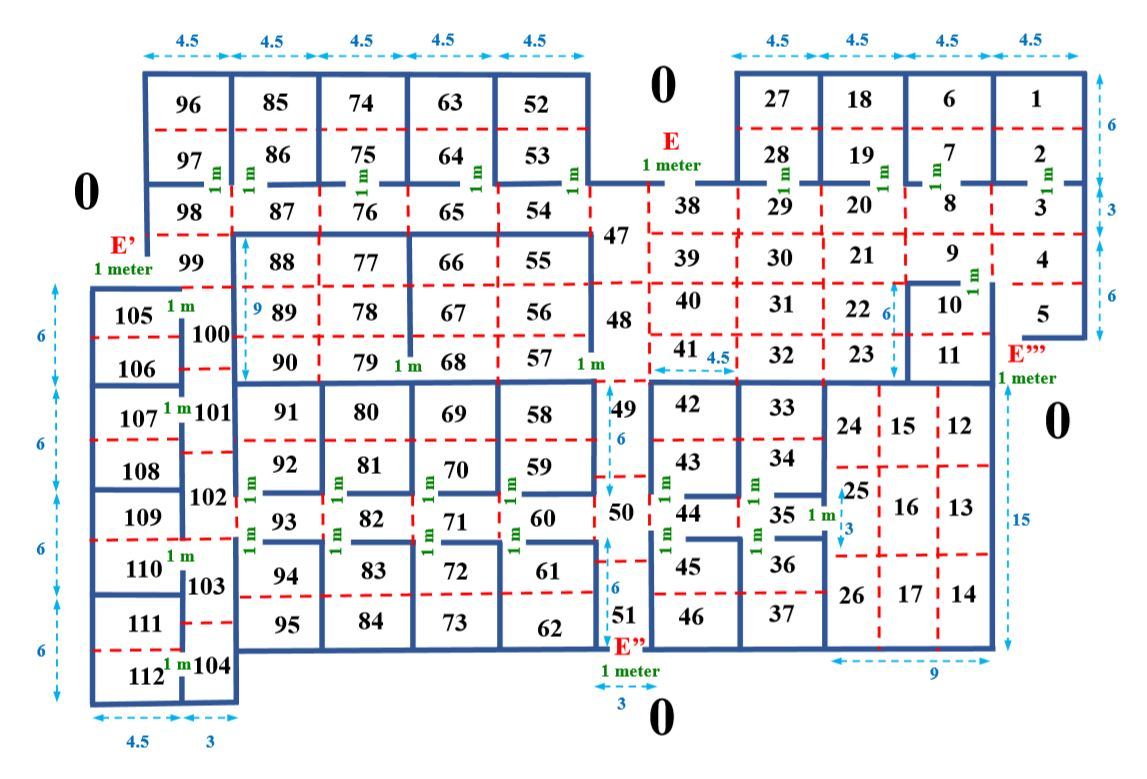
\includegraphics[scale=0.5]{implementation/coppito0.JPG}
	\caption{Coppito 0 Topological Layout}
  \label{Coppito0 layout}
\end{figure}

A detailed description of adaptation of the tool to suit the given scenario is described in the next section.

\section{PedSim Library Modules}
\label{sec: PedSim Library Modules}

The Pedism library allows for the use of pedestrian dynamics into our own software. The libpedsim simulation rendering engine can be extended, modified and modeled to suit specific behavior patterns and scenarios. The above disaster considered is fire and through this thesis, we aim to demonstrate the capabilities of this microscopic simulator, modeling crowds during an emergency evacuation using the above mentioned building topology. 

The implementation of the various scenarios(which will be explained briefly in the following section) using Pedsim is developed on Ubuntu 18.04 using libpedsim version 2.4.2.
The library itself contains many subsections and modules which handle specific tasks such as agent movement, topology description etc. The various modules of the pedsim library is described below.

The libpedsim tool can be broadly classified into 2 sections - the simulation of pedestrians and graphically rendering the simulation process onto a QT based graphical window to depict the flow of agents in real time process.

The following modules are part of rendering output to a graphical window:


\begin{enumerate}
  \item agent.h
  \item agent.cpp
  \item cell.h
  \item cell.cpp
  \item config.h
  \item config.cpp
  \item control.h
  \item control.cpp
  \item control.ui
  \item grid.h
  \item grid.cpp
  \item mainwindow.h
  \item mainwindow.cpp
  \item moc\textunderscore loadscene.cpp
  \item moc\textunderscore control.cpp
  \item moc\textunderscore mainwindow.cpp
  \item moc\textunderscore scene.cpp
  \item moc\textunderscore predefs.cpp
  \item qrc\textunderscore application.cpp
  \item scene.h
  \item scene.cpp
  \item style.h
  \item style.cpp
  \item tree.h
  \item tree.cpp
  \item ui\textunderscore control.h
\end{enumerate}

As the above modules are used to render the algorithm to a graphical output, most of the modules as mentioned above need very little to no modification whatsoever. It is also worth noting that the modules “agent.h” and “agent.cpp” contains the actual definitions for the behavior of pedestrian agents. These behavior functions are implemented by the author of the tool as a generic inter-agent based interaction and is developed keeping in mind to add further and more complex behavioral functionalities. These functions can be extended in the “ped\textunderscore agent.h” and “ped\textunderscore agent.cpp” respectively. 
The following modules below represent the core modules that we extend and modify to suit the scenario at hand:

\begin{enumerate}
  \item coppito.h
  \item coppito.cpp
  \item loadscene.h
  \item loadscene.cpp
  \item ped\textunderscore agent.h
  \item ped\textunderscore agent.cpp
  \item main.cpp
\end{enumerate}

The first two modules - “coppito.h” and “coppito.cpp” is an external module that is incorporated into the source of the libpedsim library for the specific purposes of modeling the building “Coppito 0”, as the name suggests. The detailed description of “coppito.h” and “coppito.cpp” will be listed after the brief description of the other mentioned modules. 

“loadscene” module is used to generate and extract the specific topology of the building. The exact dimensions of the building is stored on an .xml file which is then fed into the loadscene module to incorporate into the library source for graphical representation. This .xml file has specific tags which can be used to not only describe the dimensions of the building but also to specify the number of agents and the path of their trajectory - mentioned as “waypoint” within the .xml file. This information is then retrieved by the loadscene module, extract information from the various mentioned tags, and generating the mentioned number of total agens on the graphical output, adding the constrained waypoints to the agents, and most importantly, to gather the information required to generate a graph that depicts the nature of the building in description.

The “ped\textunderscore agent” module describes the behavior and movement of the agent that is to be rendered to the graphical window. This module consists of behavior functionalities that typically incorporates “social forces”, “obstacle forces”, “look ahead force”, “desired force” and “my force”. The definition of these “forces” (generic navigation constraints and behaviors) are explained below:

\begin{enumerate}
   \item my force:
   \begin{itemize}
     \item myForce() is a method that returns an "empty" force (all components set to 0). This method can be overridden in order to define own forces. This can thus be used to model more complex human navigation/decision making patterns.
   \end{itemize}
   \item lookahead force:
   \begin{itemize}
     \item This calculates the mental layer force of the strategy "look ahead". It is implemented here in the physical layer because of performance reasons.
   \end{itemize}
   \item obstacle force:
   \begin{itemize}
     \item This calculates the force between this agent and the nearest obstacle in this scene.
     \item It iterates over all obstacles.
     \item Hence the complexity of this module is equal to $O(N)$.
   \end{itemize}
   \item social force:
   \begin{itemize}
     \item This module calculates the social force between this agent and all the other agents belonging to the same scene.  It iterates over all agents inside the scene.
     \item Hence it has a complexity of $O(N^2)$.
   \end{itemize}
   \item desired force:
   \begin{itemize}
     \item This module calculates the force between this agent and the next assigned waypoint.  If the waypoint has been reached, the next waypoint in the list will be selected.
     \item At the moment, a visited waypoint is pushed back to the end of the list, which means that the agents will visit all the waypoints over and over again.
   \end{itemize}
\end{enumerate}

The main behavioral functionalities to be incorporated is thus implemented in the ped\textunderscore agent module. The agents are made to move according the complex grid geometry based architecture called \textit{Alan Turing Building Architecture} which is implemented in the “coppito” source module.

As aforementioned, the .xml file contains a generic description of the topology of the building that is to be modeled and used for rendering simulation. The coppito.xml is the file used in our case for the modeling of our present scenario. This information is retrieved by the “loadscene” module to extract the exact graphical plot points to draw the building. 

The following figure \ref{coppito_pedsim} depicts the environment of PedSim and the coppito 0 building that is modeled. 

\begin{figure}[H]
  \centering
  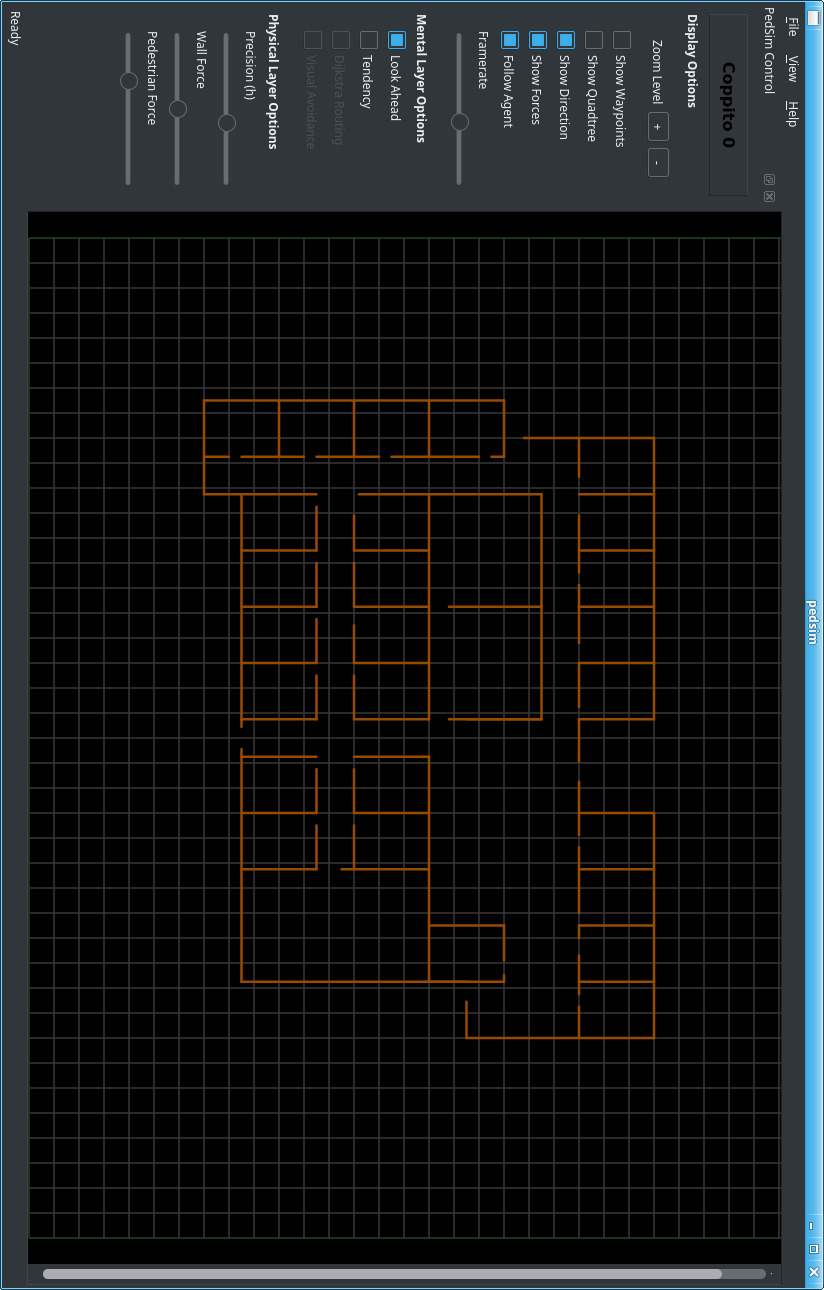
\includegraphics[scale=0.6]{implementation/coppito0building.png}
  \caption{Grid Representation of Coppito 0 within the PedSim Environment}
  \label{coppito_pedsim}
\end{figure}

\begin{figure}[H]
  \centering
  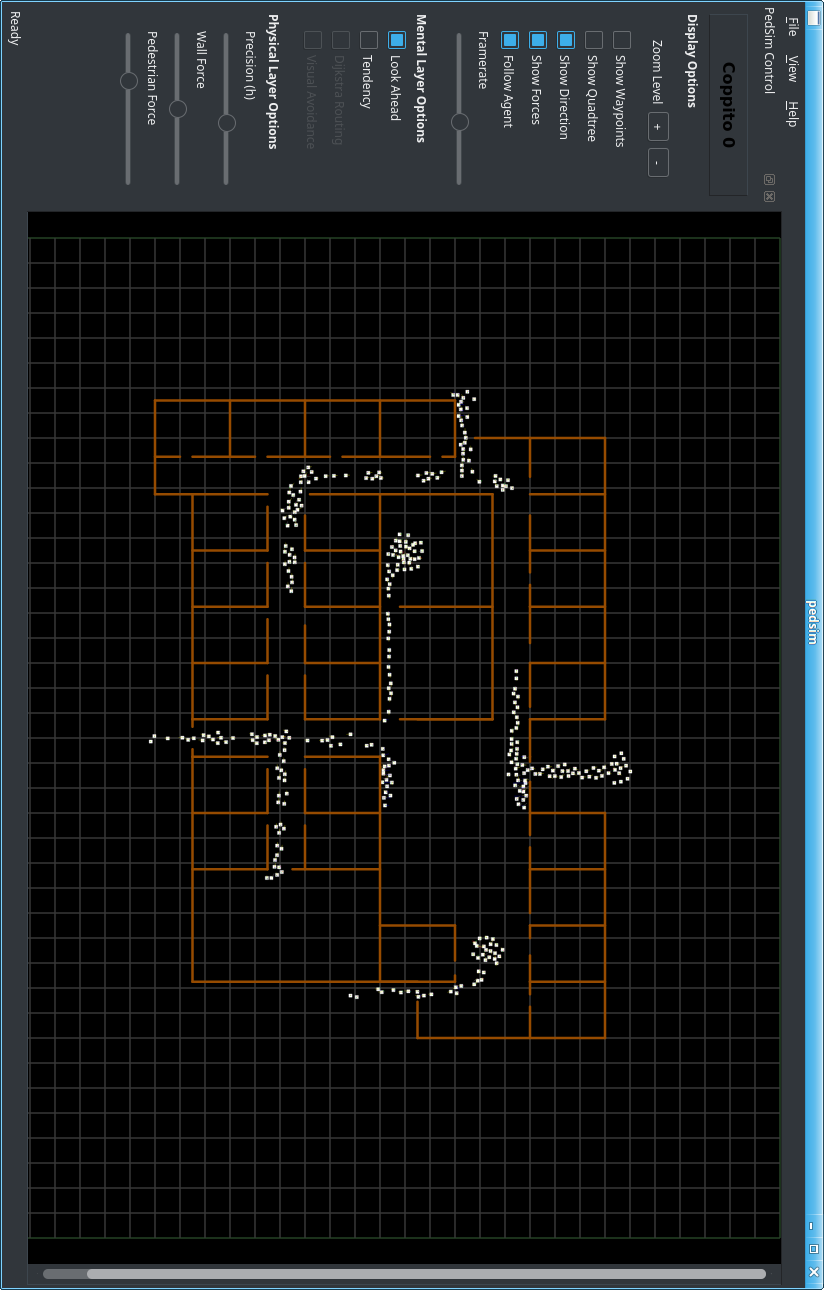
\includegraphics[scale=0.6]{implementation/simulationinaction.png}
  \caption{Microscopic Agent Simulation in PedSim}
  \label{coppito_simulation}
\end{figure}

The above figure \ref{coppito_simulation} represents the microscopic agents being simulated within the PedSim environment, as the agents are subjected to the various constraints and are tasked to evacuate to the safe zone \textbf{"E"}.

PedSim also provides a quick and easy way to change certain key constraints within its front end QT client. The following figure \ref{variableOptions} depicts the variables that can be changed in real time whilst the simulation is being processed.

\begin{figure}[H]
  \centering
  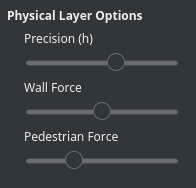
\includegraphics[scale=0.7]{implementation/variableOptions.png}
  \caption{Real Time Variable Constraints in PedSim}
  \label{variableOptions}
\end{figure}

The above figure depicts 3 variable sliders that can be applied to the simulation in real time. The three sliders are explained as follows:

\begin{enumerate}
  \item precision(h) - this represents the time steps $\tau$. These are discretized time steps that are used to calculate the total time taken for the evacuation of the participating agents.
  \item Wall Force - this force determines how close to the obstacles they can tread, this is extremely useful in modelling situations like fire, heat etc., in cases where the walls of the topology should not approached due the nature of the disaster or situation.
  \item Pedastrian Force - This force essentially determines the social forces among the participating agents. The more the pedastrian force the less intermixing happens between the agents. This variable constraint is especially important in modelling cell capacities and in determining flow dynamics. 
\end{enumerate}

The following subsection describes in detail the algorithm that is used in the simulation of the various scenarios. 


\section{Algorithm Description}
\label{sec: Algorithm Description}

All the agents within the PedSim environment are modeled and simulated according to certain realistic constraints. These constraints form the backbone that defines how the agents interact with one another and the environment that surrounds them. To make things simpler, the modeled topology is subdivided into grids. These grids are further divided into atomic square divisions of certain length and breadth. For convenience, we term these square divisions as cells. Constraints such as capacity, flow etc. are imposed on these cells to create a flow dynamic that is closer to the realistic simulation of an emergency evacuation. Within the premise of the running program, these are plot points which are manipulated by the program. 

The “coppito” module pipelines this plot information for further processing. The basic movement of agents are strictly modeled according to the algorithm presented in \cite{ref5}. Various constraints are mentioned in the paper for the anaylsis of a shortest egress path during design time. However these constraints alone are not enough to make the simulations close to be realistic. Once the basic algorithm is explained, further conditions will be introduced and explained. 

In the work by H.Muccini et. al \cite{ref5}, discussion of the linearization of the constraints for effectively reducing the evacuation time of the agents is mentioned. However since its redundant to use linearization within the pedsim framework to simulate for the scenario, we mainly consider only 3 of the below mentioned constraints.

\begin{equation}\label{eq1}
    y^t_j-y^{t-1}_j-\sum_{i:ij\in A}x^{t-1}_{ij}+\sum_{i:ji\in A}x^{t-1}_{ji}=0
\end{equation}

\hspace{100mm} $j\in V,t\in T,t>0$

\begin{equation}\label{eq2}
  0\leq x^t_{ij}+x^t_{ji}\leq c_{ij}
\end{equation}

\hspace{100mm} $t\in T,ij\in A$

\begin{equation}\label{eq3}
  0\leq y^t_i\leq n_i
\end{equation}

\hspace{100mm} $t\in T,i\in V$

Where,

\begin{enumerate}
  \item $T=\{0,1,...,\tau\}$, set of unit of time slots.
  \item $y^t_i$ = state of cell $i\in V$ at time $t\in T$, that is, the number of persons that occupy $i$ at $t$.
  \item $n_i$ = capacity of cell $i$; it measures the maximum nominal amount of people that $i$ can host at any time.
  \item $x^t_{ij}$ = how many persons move from cell $i$ to an adjacent cell $j$ in $(t, t+1]$; this gives the average speed at which the agent flow proceeds from cell $i$ to cell $j$.
  \item $c_{ij}$ = capacity of the passage between cell $i$ and cell $j$; this is the maximum amount of people that, independently on how many persons there are in cell $j$, can traverse the passage in the time unit.
\end{enumerate}

The above conditions are a set of mandatory inclusive pre-requisites required to be included from \textit{An IoT Software Architecture for an Evacuable Building Architecture} by H. Muccini et. al \cite{ref5}, since the experimentation of various scenarios are based on the aforementioned set of equations and conditions. Through this thesis we introduce 4 more constraints to be included along with this base algorithm. The specific nature and details of the additional constraints will be discussed in the next chapter, where the various different experiments and scenarios are carried and are analyzed. It must also be mentioned that in order to be coherent with the mentioned work and also to analyze optimal egress paths the following condition is also considered in addition to the above 3:


\hspace{60mm} max $y^\tau_0$    \hspace{60mm} (3.4)

The above condition is obviously included in order to maximize the number of evacuees during the disaster scenario.


\section{Topology Formulation}
\label{sec: Topology Formulation}


The topology of the building as given in \ref{Coppito0 layout} is modeled according to the \textit{Alan Turing Building Architecture} and as shown in the figure the whole Coppito 0 building is subdivided into cells of equal length and breadth. Each cell also has a cell capacity as defined above and is assumed that inter-connected cells have full passage, if not bound by walls or walls with reduced passage capacity(doors). 

The coppito source module divides the entire topology into such grids that are composed of cells, whose initial plot point is taken from the loadscene module, which in turn takes its information from the coppito.xml file. To translate simple plot points to a complex cell based grid structure, a highly complex user defined data structure was developed to store this information. 

The plot points that are stored into the .xml file is randomly plotted with the exception of the first starting point in order to facilitate a quicker render of the entire building. However for the processing of a cell based structure, this information cannot be random and hence the information is then once again converted to form a structured cell geometry.

Thus a complex user defined data structure is defined to hold all this information in place. For the sake of convenience and optimal storage of data, the coppito 0 building is divided into regions called blocks. Each block contains a set number of cells and naturally have a variable number of cells. The whole topology is divided into 18 blocks and consists in total of 119 cells. Each cell is also of a specific dimension and has a certain cell length and a cell width. To understand what a block is, it can be easily explained diagrammatically as follows:

\begin{figure}[H]
  \centering
  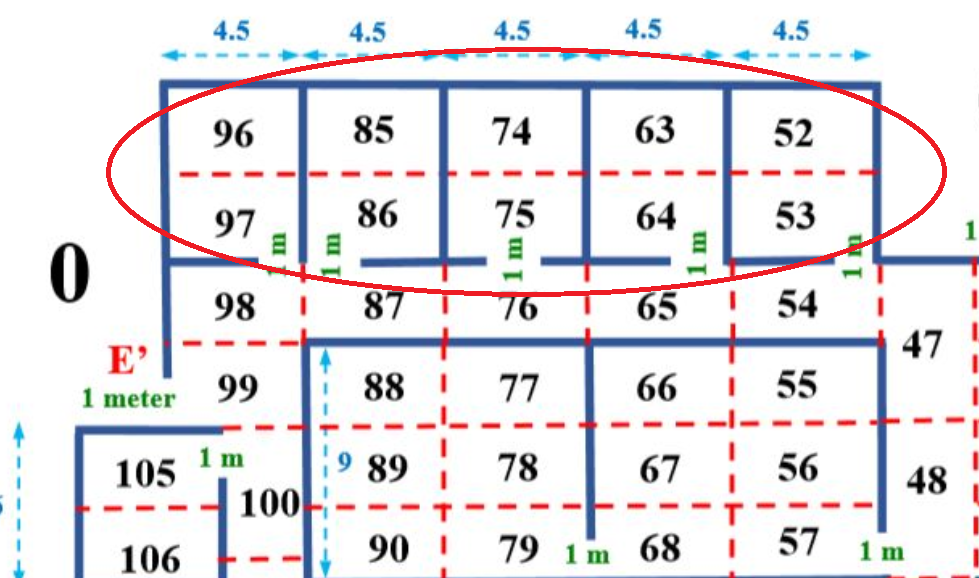
\includegraphics[scale=0.5]{implementation/block.png}
  \caption{Groups of Cells Making a Block Structure}
  \label{block}
\end{figure}

From the above figure \ref{block}, the red encircled circled area which includes the cells numbered 96, 85, 74, 63, 52, 97, 86, 75, 64, 53 form a block. Although a certain number of cells make up a block, the number of cells that make a block is often variable. Essentially one section of the topology is considered a block. This helps segregate different areas of the premises and identify them easily.

Further decomposing the cell, subdivides it into 4 edge lines, each edge line further decomposes into 4 vertices, an end to end $x$ and $y$ plot points. Along with these information are stored if the edge lines are walls and if they incorporate doors. This is highly useful for creating a tree structure pattern for path finding, used by agents during evacuation simulation. The final complex structure that is defined to hold this cell structure is explained in detail in the Appendix section. In order to dynamically store the data of the cell information, the data structure used in place is a custom user defined 7 layered structure. 

There are several sub-modules implemented in this custom made source file. The following are the following methods that are implemented as part of the module:

\begin{enumerate}
  \item divide\textunderscore cells
  \item cell\textunderscore structure\textunderscore allocation
  \item vertical\textunderscore cell\textunderscore allocation
  \item non\textunderscore standard\textunderscore vertical\textunderscore allocation
  \item wall\textunderscore allocation
  \item wall\textunderscore division\textunderscore horizontal
  \item wall\textunderscore division\textunderscore vertical
  \item door\textunderscore allocation
  \item graph\textunderscore tree\textunderscore structuring
  \item print\textunderscore block
  \item print\textunderscore walls
  \item print\textunderscore door
  \item print\textunderscore graph
\end{enumerate}

Further details regarding the technical and programmatic implementation of these modules are provided in the Appendix section of the thesis. The following section discusses the modification to the existing unoptimized algorithm from \cite{ref5}. The different simulation results comparing macro and micro agent simulations are presented and analyzed. The resulting the implications of these observations are discussed. 
 

